\section{Temperature Uniformity of the Systems att C200-40 Cold Chuck}
\label{appendix:chuck_temp}
The leakage current in silicon devices is dependent on the temperature.
For the investigated sensors in this work, the current is mainly generated in the bulk for which the temperature ($T$) and current ($I$) are related by~\ref{eq:temp_scaling}~\cite{Chilingarov_2013}, where $E_\text{eff}=\SI{1.21}{\electronvolt}$ is the effective gab energy and $k_b$ denotes the Boltzmann constant.
\begin{equation}
    \frac{I}{T^2}\cdot \exp{\frac{E_\text{eff}}{2\cdot k_b \cdot T}}~\equiv~\text{const.}
    \label{eq:temp_scaling}
\end{equation}
The validity of this temperature scaling law applied for the HGCAL silicon pad sensors in the relevant temperature range has been verified and is illustrated in~\ref{plot:iv_tempscaling}.
\begin{figure}
	\centering
	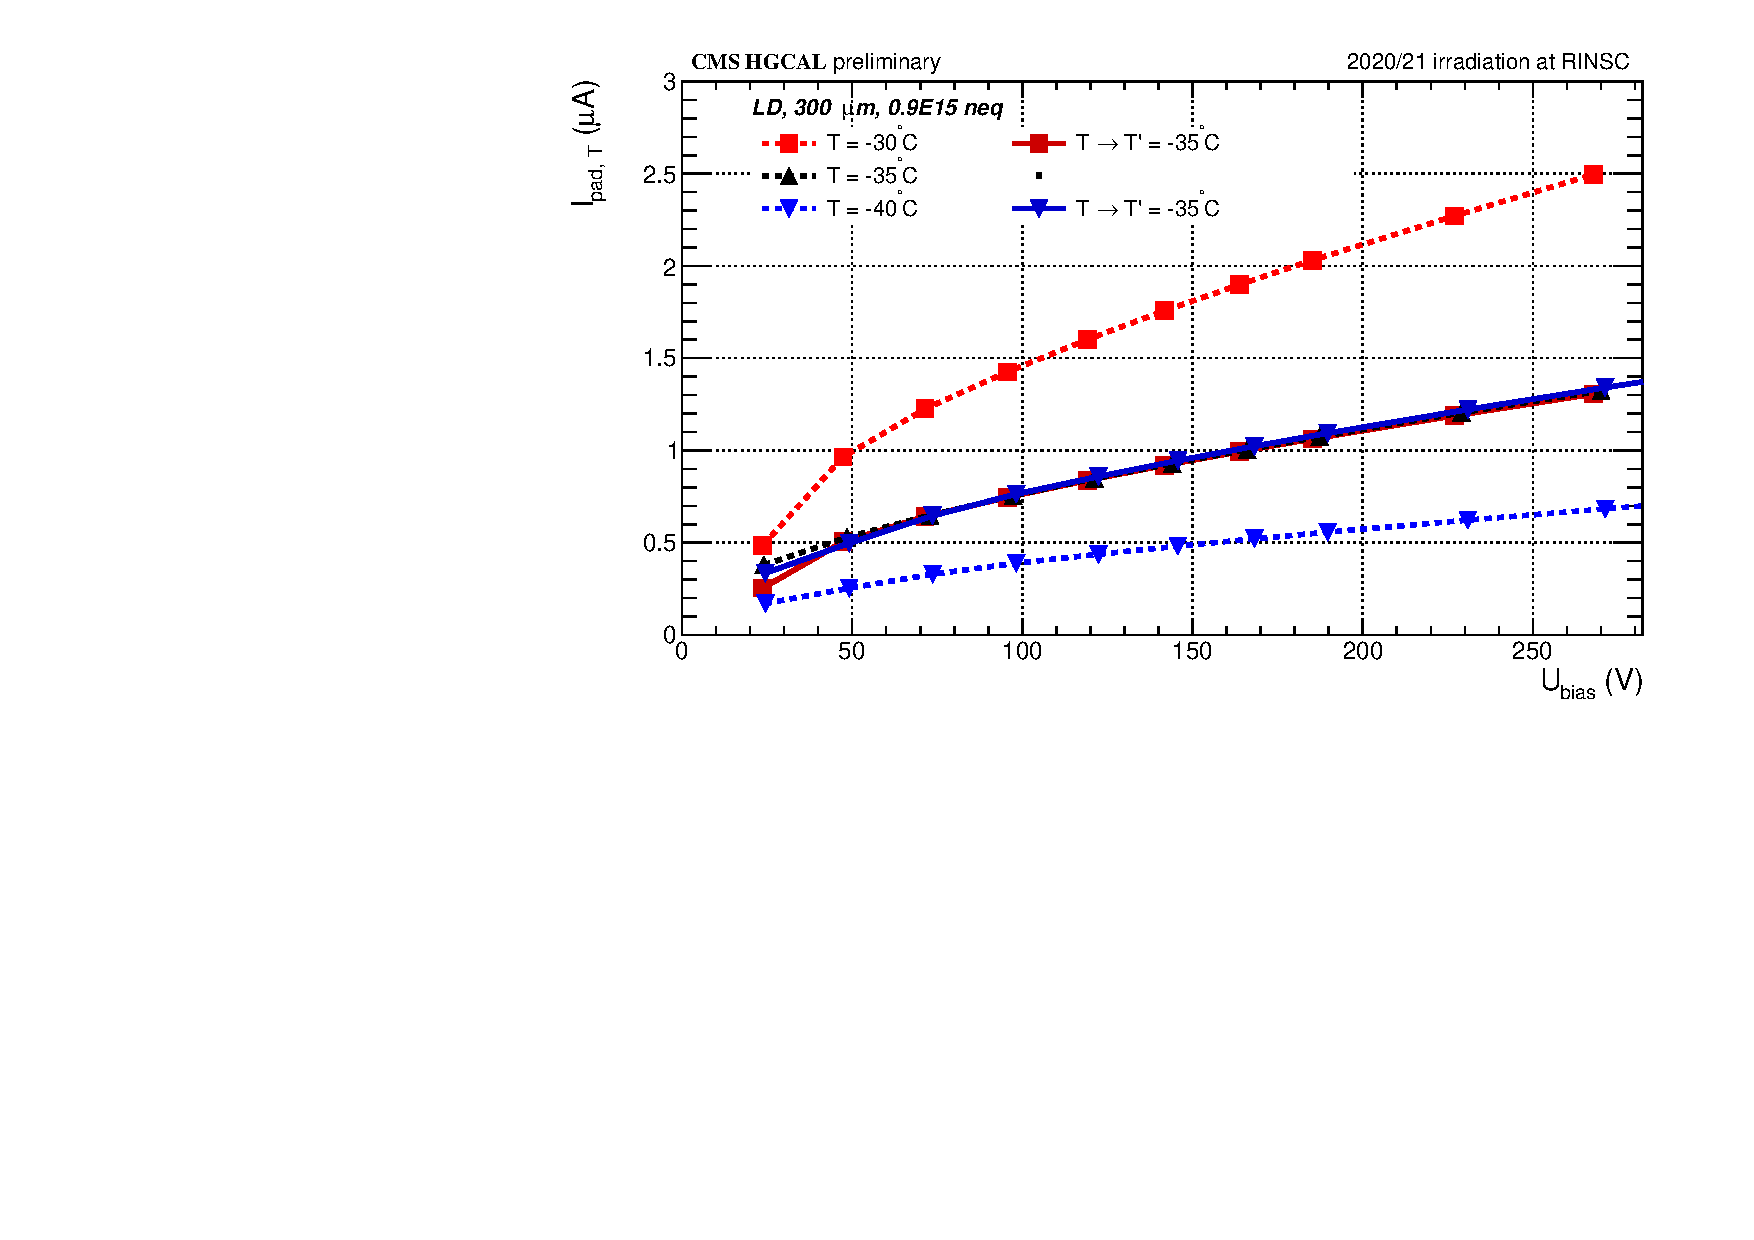
\includegraphics[width=0.69\textwidth]{plots/iv_temp_scaling/iv_overlay_ch24.pdf}
	\caption{
		Leakage currents as a function of the bias voltage for an example sensor measured at \SI{-40}{\celsius}, \SI{-35}{\celsius}, \SI{-30}{\celsius}, and scaled to \SI{-35}{\celsius} using$~$\ref{eq:temp_scaling}.
		}
	\label{plot:iv_tempscaling}
	\end{figure}
Notably, a change by \SI{1}{\celsius} impacts the current by more than 10$~\%$. 
Variations of the temperature across the chuck, and with it across the sensor, may mimic neutron fluence profiles as in~\ref{plot:iv_hexplot}. 
Thus, they should be identified and corrected for.%\newline
In this work, the temperature non-uniformity of the cold chuck at CERN (C200-40 model produced by Systems att) could be estimated from leakage current data of neutron-irradiated sensors.
By comparing per-pad currents ($I_{i(j,k)}$) at a fixed bias voltage between symmetric locations $i$, $j$, $k$, temperature differences $\delta I_{i(j), k}$ can be calculated according to~\ref{eq:temp_diff}.
For this purpose, one of the neutron-irradiated low density sensors was characterised three times at \SI{0}{\degree}, \SI{120}{\degree}, and \SI{240}{\degree} orientation.
The precision in repeating the sensor placement on the chuck can be neglected with respect to the size of the pads. 
\begin{equation}
    \frac{\delta I_{i(j),k}}{I_k} = \frac{\delta T_{i(j), k}}{T_k} \cdot \left(2 + \frac{E_\text{eff}}{2\cdot k_b \cdot T_k} \right)~,~~T_k \coloneqq T_\text{ref}
    \label{eq:temp_diff}
\end{equation}
\ref{plot:chucktemp_before} shows the hereby computed chuck temperature differences.
The determined variation is consistent with the $\pm\SI{0.5}{\celsius}$ non-uniformity as specified by the chuck producer.
Assuming a reference temperature of $T_\text{ref}\equiv\SI{-40}{\celsius}$, a two-dimensional gaussian parameterisation bound to $[\SI{-0.5}{\celsius}, \SI{0.5}{\celsius}]$ is fitted to reproduce the temperature differences $\delta I_{i(j),k}$.
The fit is performed with the tensorflow library (version 2.6.0) and the result is shown in~\ref{plot:chucktemp_correction}.
\begin{figure}
	\captionsetup[subfigure]{aboveskip=-1pt,belowskip=-1pt}
	\centering
	\begin{subfigure}[b]{0.32\textwidth}
		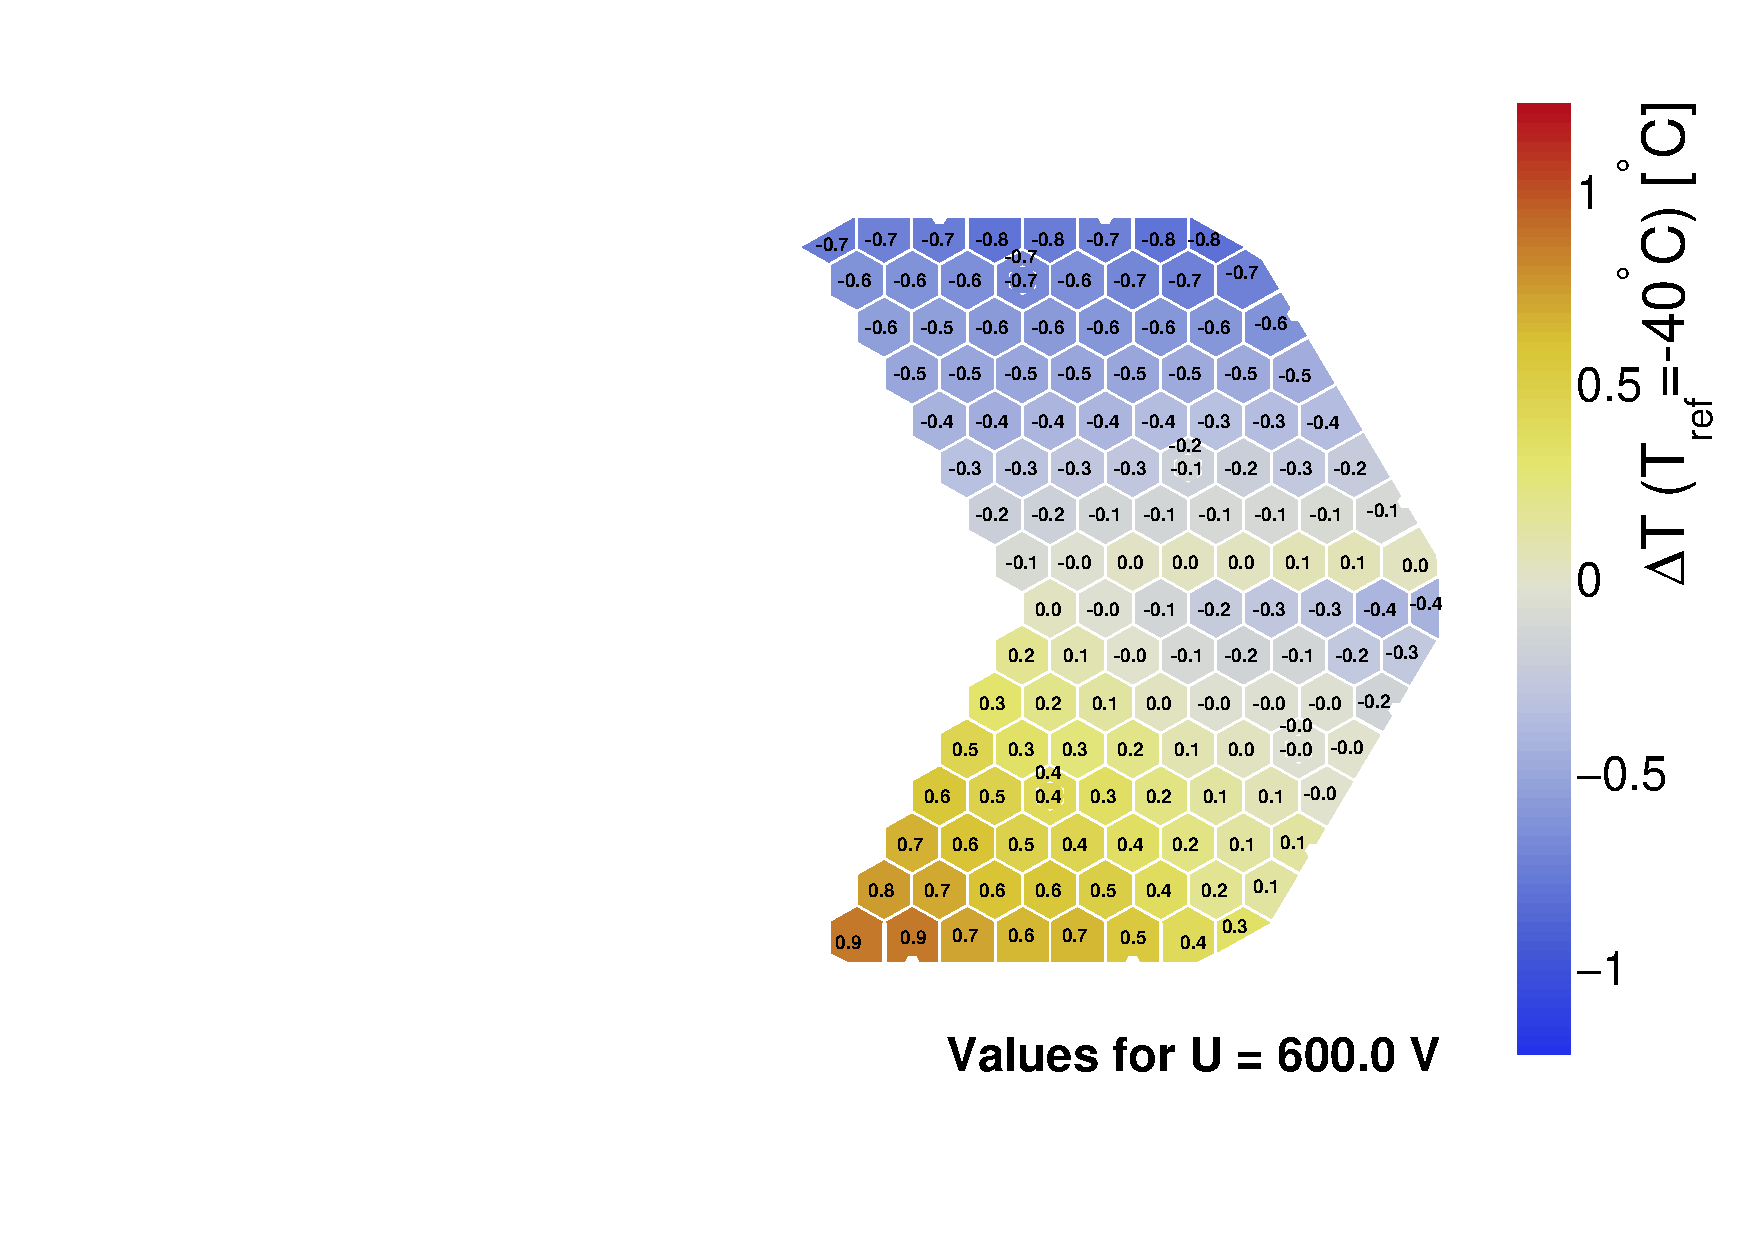
\includegraphics[width=0.999\textwidth]{plots/chuck_temp_correction/Spring2021_ALPS.pdf}
		\subcaption{
		}
		\label{plot:chucktemp_before}
	\end{subfigure}
	\hfill
	\begin{subfigure}[b]{0.32\textwidth}
		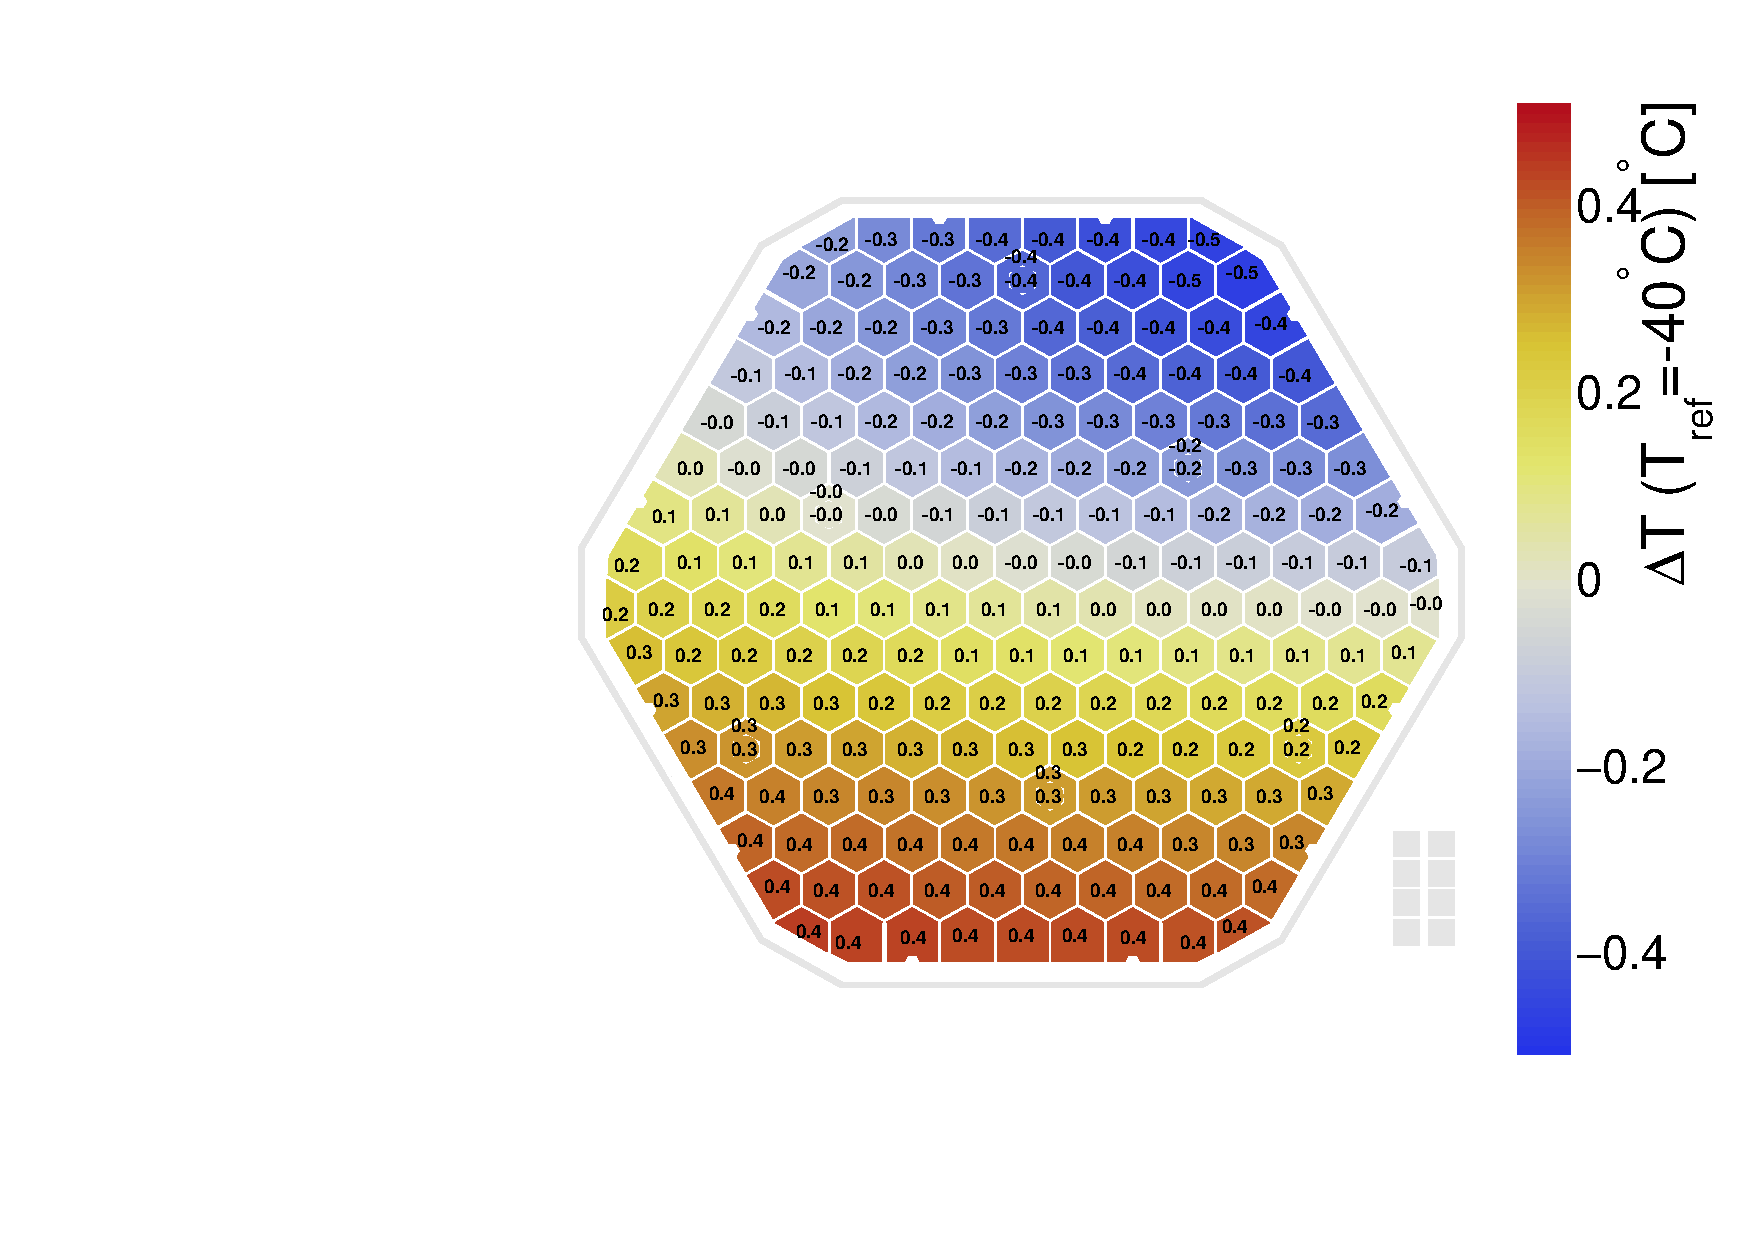
\includegraphics[width=0.999\textwidth]{plots/chuck_temp_correction/Spring2021_ALPS_deltaT.pdf}
		\subcaption{
		}
		\label{plot:chucktemp_correction}
	\end{subfigure}
	\hfill
	\begin{subfigure}[b]{0.32\textwidth}
		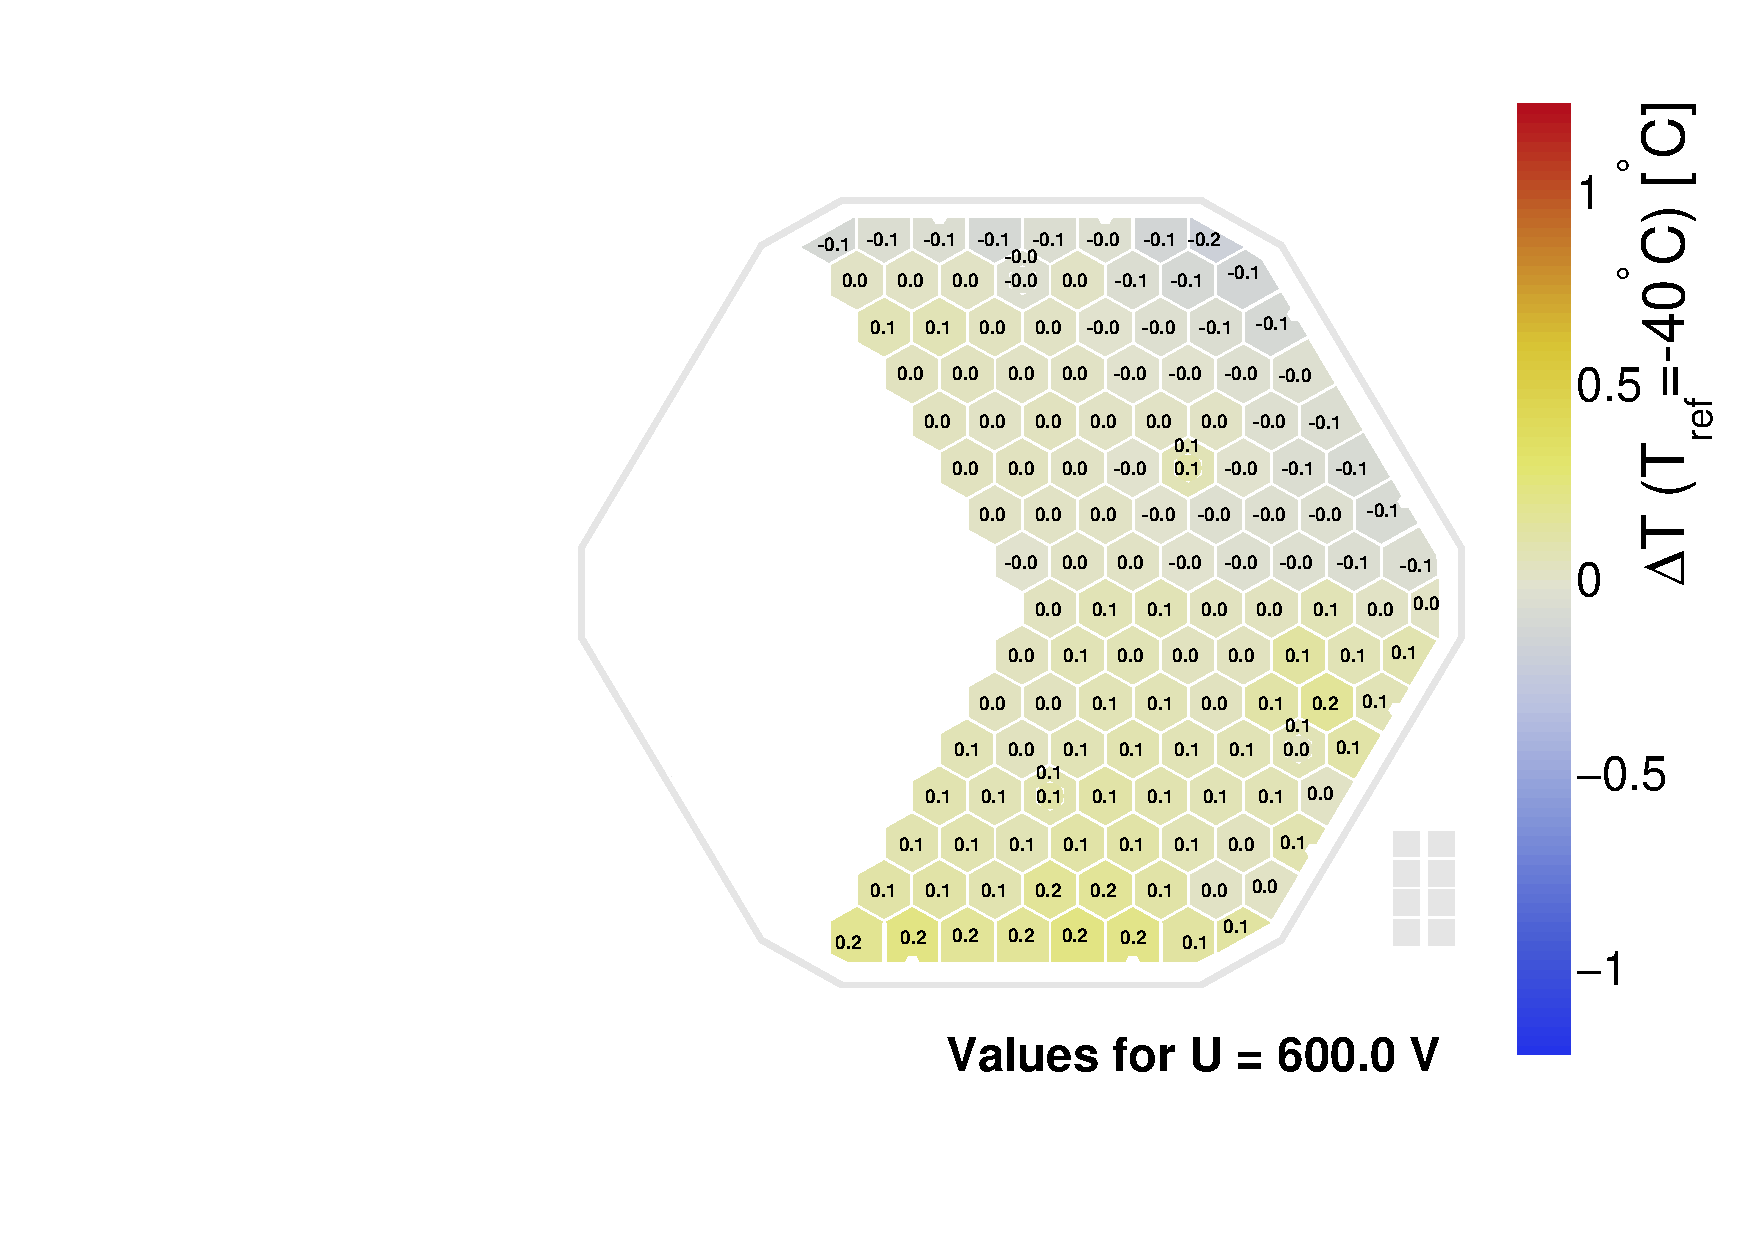
\includegraphics[width=0.999\textwidth]{plots/chuck_temp_correction/Spring2021_ALPS_chucktempcorrected.pdf}
		\subcaption{
		}
		\label{plot:chucktemp_after}
	\end{subfigure}
	\caption{
		(a) Temperature differences derived from per-pad leakage currents between symmetric locations of a representative neutron-irradiated HGCAL silicon sensors on the cold chuck at CERN.
		(b) Determined profile of temperature differences, modelled as a two-dimensional gaussian, across the sensor surface.
		(c) Closure check: derived temperature differences after accordingly correcting the measured per-pad leakage currents.
	}
\end{figure}
The hereby constructed map of chuck temperature differences is input to correct the measured per-pad leakage currents using~\ref{eq:temp_scaling}.
As a closure check, the re-application of~\ref{eq:temp_diff} on the temperature-corrected dataset demonstrates the applicability of this particular chuck temperature model.
